% This program is free software: you can redistribute it and/or modify it under the terms of the GNU General Public License as published by the Free Software Foundation, either version 3 of the License, or (at your option) any later version.
%
% This program is distributed in the hope that it will be useful, but WITHOUT ANY WARRANTY; without even the implied warranty of MERCHANTABILITY or FITNESS FOR A PARTICULAR PURPOSE. See the GNU General Public License for more details.
%
% You should have received a copy of the GNU General Public License along with this program. If not, see <https://www.gnu.org/licenses/>.

\documentclass[10pt]{beamer}

\usetheme[progressbar=frametitle, numbering=fraction, background=dark]{metropolis}
\usepackage{appendixnumberbeamer}

\usepackage{booktabs}
\usepackage[scale=2]{ccicons}

\usepackage{hyperref}
\usepackage{multimedia}
% \usepackage{media9}

\usepackage{enumerate}
\usepackage[skip=2pt]{caption}

\usepackage{multimedia}
\usepackage{minted}

% This program is free software: you can redistribute it and/or modify it under the terms of the GNU General Public License as published by the Free Software Foundation, either version 3 of the License, or (at your option) any later version.
%
% This program is distributed in the hope that it will be useful, but WITHOUT ANY WARRANTY; without even the implied warranty of MERCHANTABILITY or FITNESS FOR A PARTICULAR PURPOSE. See the GNU General Public License for more details.
%
% You should have received a copy of the GNU General Public License along with this program. If not, see <https://www.gnu.org/licenses/>.

\documentclass[10pt,presentation]{beamer}

\usetheme[progressbar=frametitle, numbering=fraction, background=dark]{metropolis}
\usepackage{appendixnumberbeamer}

\usepackage{booktabs}
\usepackage[scale=2]{ccicons}

\usepackage{hyperref}
\usepackage{multimedia}

\usepackage{enumerate}
\usepackage[skip=2pt]{caption}

\usepackage{dirtytalk}
\usepackage{multimedia}
\usepackage[outputdir=build]{minted}

\usepackage{tikz}
\usepackage{tikzducks}
\usepackage{bookmark}

% https://tex.stackexchange.com/questions/152392/date-format-yyyy-mm-dd
\usepackage[yyyymmdd]{datetime}
\renewcommand{\dateseparator}{--}

% Copied from https://github.com/matze/mtheme/blob/master/source/beamerinnerthememetropolis.dtx
\setbeamertemplate{title page}{
  \begin{minipage}[b][\paperheight]{\textwidth}
    \vfill%
    \ifx\inserttitle\@empty\else\usebeamertemplate*{title}\fi
    \ifx\insertsubtitle\@empty\else\usebeamertemplate*{subtitle}\fi
    \usebeamertemplate*{title separator}
    \ifx\inserttitlegraphic\@empty\else\usebeamertemplate*{title graphic}\fi
    \ifx\beamer@shortauthor\@empty\else\usebeamertemplate*{author}\fi
    \ifx\insertdate\@empty\else\usebeamertemplate*{date}\fi
    \ifx\insertinstitute\@empty\else\usebeamertemplate*{institute}\fi
    \vfill
    {\tiny Copyright (C) 2023 Jamal Bouajjaj under GPLv3} \par
    \vspace*{5mm}
    \vspace*{1mm}
  \end{minipage}
}

\setbeamertemplate{title graphic}{
  \vbox to 0pt {
    \vspace*{0em}
    \inserttitlegraphic%
  }%
  \nointerlineskip%
}

\titlegraphic{\hfill \begin{tikzpicture}[scale=0.75]
\duck[magichat,magicwand,magicstars=blue!60!white,squareglasses=blue!50!black]
\end{tikzpicture}}

\newenvironment{Figure}
  {\par\medskip\noindent\minipage{\linewidth}\centering}
  {\endminipage\par\medskip}

\newcommand\Wider[2][3em]{%
\makebox[\linewidth][c]{%
  \begin{minipage}{\dimexpr\textwidth+#1\relax}
  \raggedright#2
  \end{minipage}%
  }%
}


\title{Lecture \#4: Git SCM}
\date{\today}
\author{Presented by Jamal Bouajjaj}
\institute{For University of New Haven's Fall 2023 CSCIxx51 Course}

% From https://tex.stackexchange.com/questions/66519/make-each-frame-not-slide-appear-in-the-pdf-bookmarks-with-beamer
\makeatletter
\apptocmd{\beamer@@frametitle}{\only<1>{\bookmark[page=\the\c@page,level=3]{#1}}}%
% {\message{** patching of \string\beamer@@frametitle succeeded **}}%
% {\message{** patching of \string\beamer@@frametitle failed **}}%
\makeatother

% From https://tex.stackexchange.com/questions/471117/how-to-add-the-source-of-the-current-page-to-the-footer-in-a-beamer-theme
\renewcommand{\footnoterule}{}
\setbeamercolor{framesource}{fg=gray}
\setbeamerfont{framesource}{size=\tiny}

\defbeamertemplate{footnote}{unnumbered}{%
    \usebeamercolor[fg]{framesource}%
    \usebeamerfont{framesource}%
    \hfill\insertfootnotetext%
}

\newcommand{\Imgsource}[1]{%
    \setbeamertemplate{footnote}[unnumbered]%
    \footnotetext{Image Source: \url{#1}}%
}

\begin{document}

\maketitle

\section{Intro}

\begin{frame}{Git}
  Git is a Source-Control Management (SCM) system.

  Started by Linus Torvalds himself, it is the most widely used version control software.
\end{frame}

\begin{frame}{How popular?}
    From \url{https://openhub.net/repositories/compare}:
    \centering 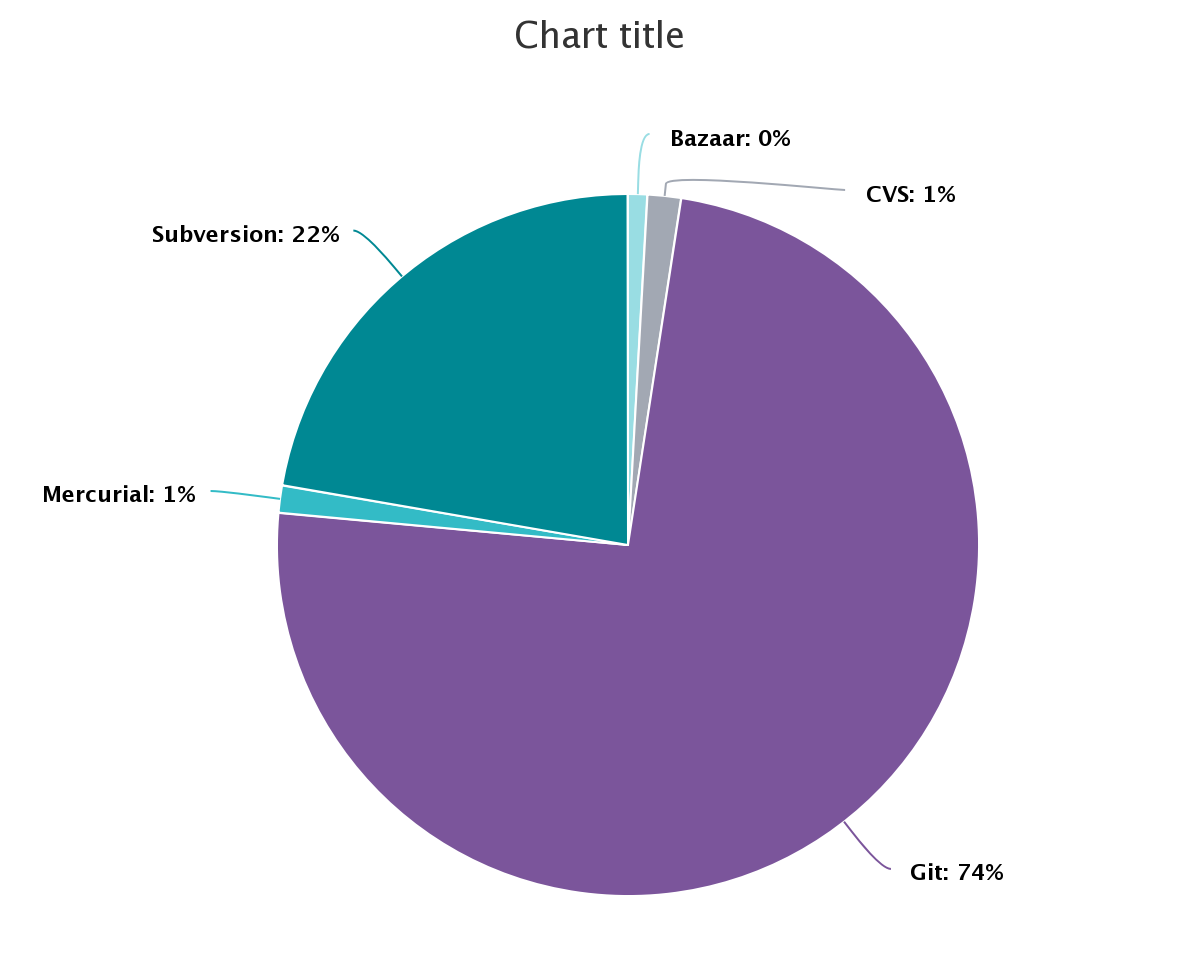
\includegraphics[height=0.8\textheight]{eimg/gitpop.png}
    \Imgsource{https://openhub.net/repositories/compare}
\end{frame}

\begin{frame}{So Github?}
    Q: \textit{So is this just Github?} \pause

    A: \textbf{NO}

    \vspace{2em}
    While Git and Github is related, the former is the version control software, and the latter is a really nice git server.
\end{frame}

\begin{frame}{Why??}
    \begin{itemize}[<+->]
        \item For tracking changes throughout a project
        \item For making changes to code with a team or world-wide
        \item For blaming bad code (git blame)
    \end{itemize}
\end{frame}

\section{Installation}

\begin{frame}{Installation}
    It can be downloaded from \url{https://git-scm.com/}. The setup process is pretty easy.
\end{frame}

\begin{frame}{Free Book and Cheat Sheet}
    If you want a good reference, there is a free book that can be downloaded right from git's webpage. There is also a cheat sheet for quick command references:

    \url{https://git-scm.com/book/en/v2}

    \url{https://training.github.com/downloads/github-git-cheat-sheet.pdf}
\end{frame}

\section{Concepts}

\begin{frame}{Decentralized}
    If you have a git repo, you have it's entire history since it's inception!
    This makes it decentralized: you are not reliant on some centralized server, rather it's a convenience.
\end{frame}

\begin{frame}{Some terminology}
    \begin{itemize}
        \item \textbf{Commit}: A snapshot in time of your tracked files
        \item \textbf{Tracked Files}: Files which git will look at. All others are ignored
        \item \textbf{Branch}: Think of your repo as a tree. A branch is just that, but of code
        \item \textbf{Remote}: The server the changes are pushed unto
    \end{itemize}
\end{frame}

\begin{frame}{Files Before Commit}
    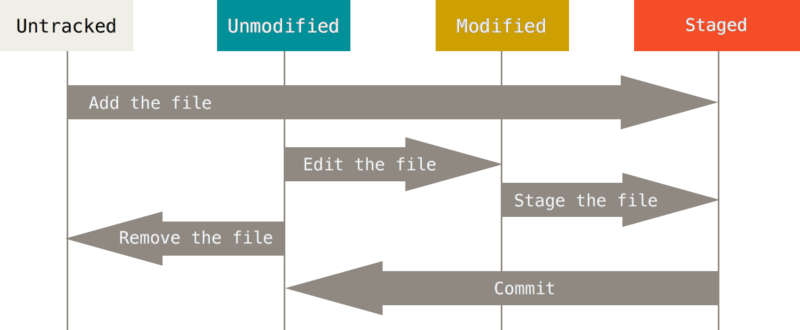
\includegraphics[width=\textwidth]{eimg/lifecycle.png}
    Some files can also be ignored with a .gitignore file
    \Imgsource{https://www.git-scm.com/book/en/v2/Git-Basics-Recording-Changes-to-the-Repository}
\end{frame}

\section{Github Workflows}

\begin{frame}{Flows}
    How you organize your branching and structure depends on your preference. There are two main schools of thought regarding this:
\end{frame}

\begin{frame}{Git Flow}
    \centering 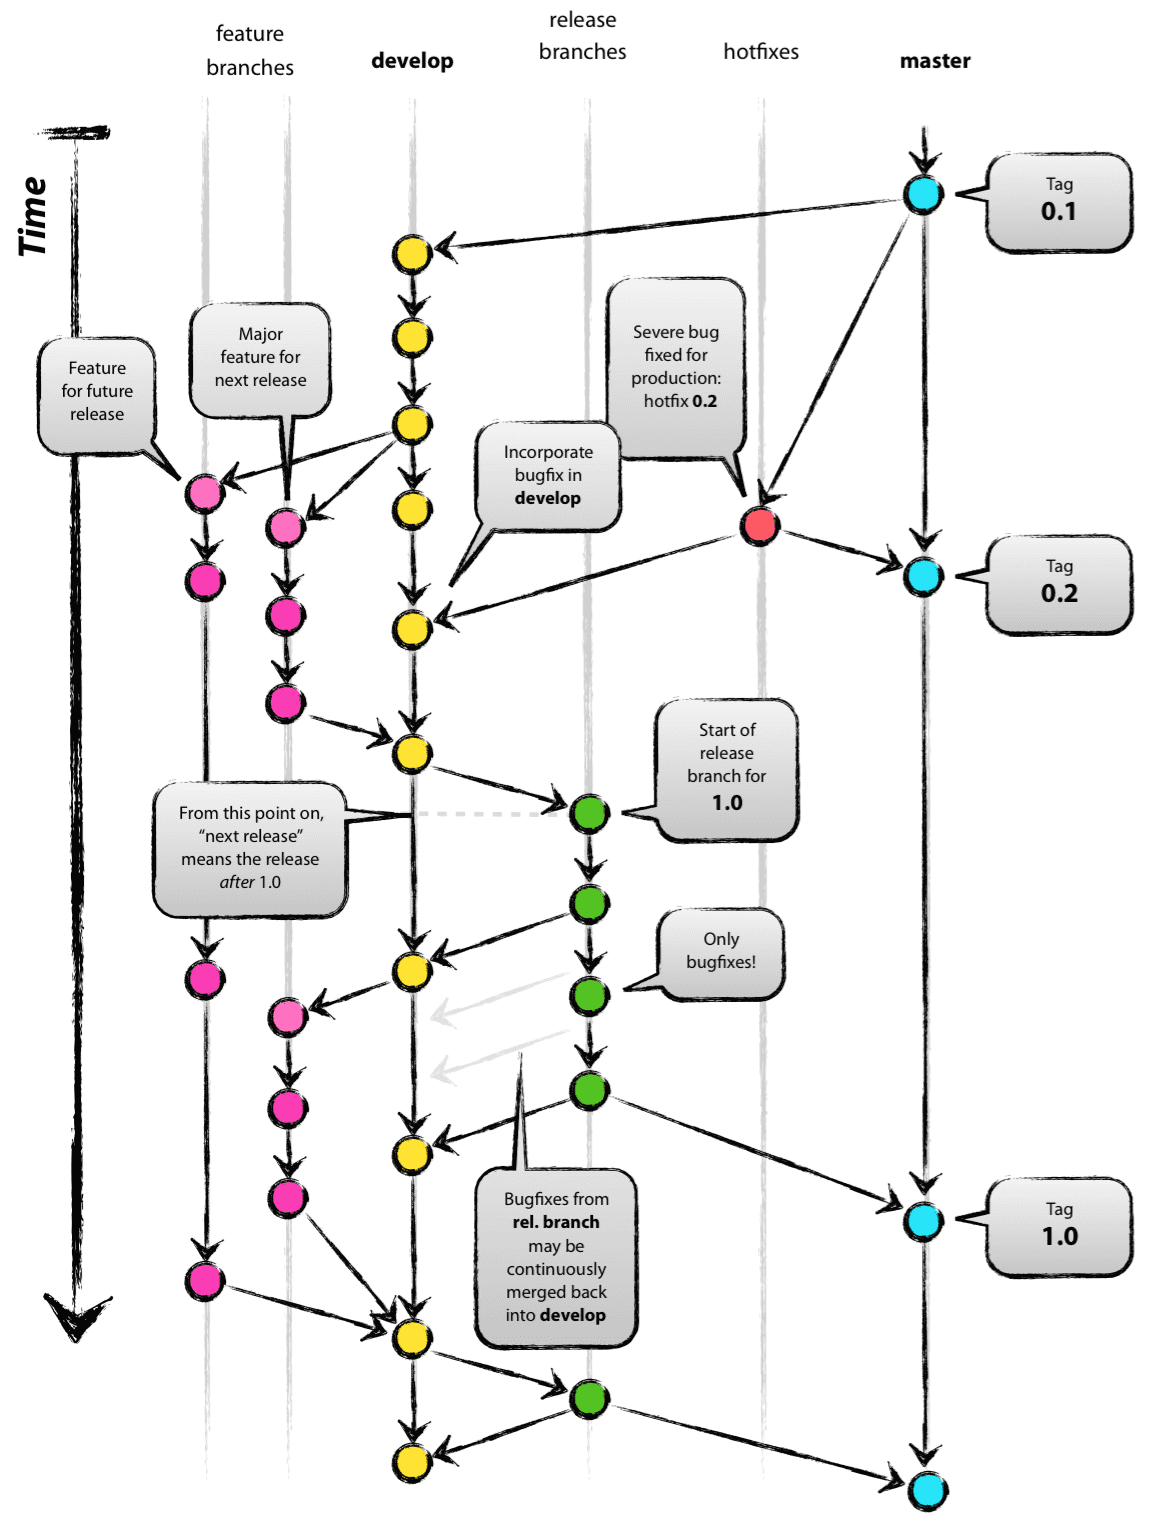
\includegraphics[height=0.8\textheight]{eimg/git-model@2x.png}
    \Imgsource{https://nvie.com/posts/a-successful-git-branching-model/}
\end{frame}

\begin{frame}{Gitub Flow}
    \centering 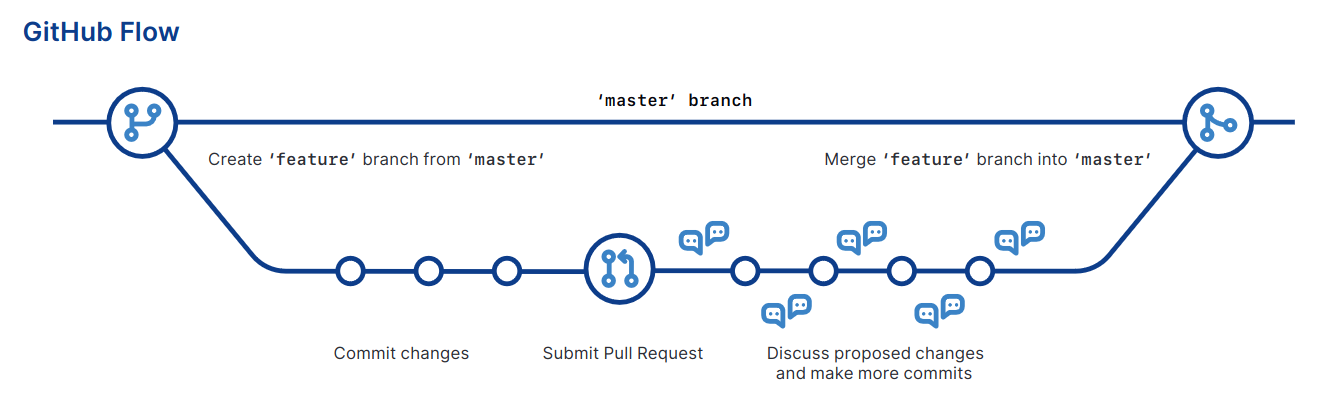
\includegraphics[width=\textwidth]{eimg/Screenshot_20230902_164537.png}
    \Imgsource{https://training.github.com/downloads/github-git-cheat-sheet.pdf}
\end{frame}

\begin{frame}{Commands}
    See cheat sheet by Github (it's actually nice!)
\end{frame}

\begin{frame}{PyCharm}
    PyCharm has git integrated into it, and we'll be demo-ing it in class!
\end{frame}

\begin{frame}{Good practices}
    \begin{itemize}
        \item Commit often
        \item Add useful commit messages
        \item If working on a team, it's better to have individual development branches that gets merged and pulled from a master branch.
        \item Only track source code: all generated stuff can be generated from the code
        \item Don't track IDE settings unless they are really needed (for example .idea)
    \end{itemize}
\end{frame}

\begin{frame}[standout]{End}
  The end
\end{frame}

\end{document}
